%% =====================================================================
%% Artigo de reprodução/replicação — INF2005 (PUC-Rio, 2026.2)
%% Estudo original: Galindo et al., SPLC'23, DOI 10.1145/3579027.3608973
%% Compilar:  make        (pdflatex + bibtex)   |   Overleaf: main.tex
%% =====================================================================
\documentclass[sigconf,nonacm]{acmart}

\usepackage[brazilian]{babel}
\usepackage[utf8]{inputenc}
\usepackage{booktabs}
\usepackage{multirow}
\usepackage{xcolor}
\usepackage{listings}
\usepackage[capitalise,nameinlink,brazilian]{cleveref}

% Figuras geradas pelo notebook ficam em 3.results/figures (raiz do repo)
\graphicspath{{figuras/}{../../3.results/figures/}}

% ---- Marcadores de trabalho (remover antes da entrega) ----
\newcommand{\todo}[1]{\textcolor{red}{\textbf{[TODO: #1]}}}
\newcommand{\felipe}[1]{\textcolor{blue}{\textbf{[Felipe: #1]}}}
\newcommand{\gabriela}[1]{\textcolor{teal}{\textbf{[Gabriela: #1]}}}
\newcommand{\leo}[1]{\textcolor{orange}{\textbf{[Leo: #1]}}}

% ---- Macros do domínio ----
\newcommand{\uvl}{UVL}
\newcommand{\flamapy}{Flamapy}
\newcommand{\RQ}[1]{\textbf{RQ#1}}

\lstdefinelanguage{UVL}{morekeywords={features,constraints,mandatory,optional,alternative,or,namespace,imports,include},sensitive=true}
\lstset{basicstyle=\ttfamily\footnotesize,keywordstyle=\bfseries,tabsize=4,breaklines=true,frame=single,columns=fullflexible}

\begin{document}

\title{LLMs para gerar instâncias significativas de feature models:\\ um estudo de reprodução e replicação}

\author{Felipe Frighetto Gonzalez}
\affiliation{\institution{PUC-Rio}\city{Rio de Janeiro}\country{Brasil}}
\email{TODO@inf.puc-rio.br}

\author{Gabriela Soares de Moraes}
\affiliation{\institution{PUC-Rio}\city{Rio de Janeiro}\country{Brasil}}
\email{TODO@inf.puc-rio.br}

\author{Leo Land Bairos Lomardo}
\affiliation{\institution{PUC-Rio}\city{Rio de Janeiro}\country{Brasil}}
\email{TODO@inf.puc-rio.br}

\renewcommand{\shortauthors}{Gonzalez, Moraes e Lomardo}

\begin{abstract}
\textbf{Contexto.} Avaliar ferramentas de análise automatizada de feature models exige muitos modelos realistas, que raramente são publicados. Galindo et al.~\cite{galindo2023llm} propuseram usar um LLM (Codex) para estender modelos reais em \uvl{}, preservando sintaxe e domínio.
\textbf{Objetivo.} Reproduzir a análise do estudo original com os artefatos publicados e replicá-lo com LLMs atuais.
\textbf{Método.} \todo{resumir: reprodução com as 150 respostas do Codex; replicação com 1 LLM via API e 1 local, instruction prompting, avaliação em funil (sintaxe, lógica, estrutura, domínio).}
\textbf{Resultados.} Na reprodução, 136 de 150 variantes (90,7\%) são sintaticamente válidas, como no artigo; porém a similaridade de domínio mediana nos dados publicados é 0,94, acima da faixa 0,5--0,8 relatada. \todo{resultados da replicação: RQ1--RQ4.}
\textbf{Conclusão.} \todo{}
\end{abstract}


\keywords{large language models, feature models, UVL, reprodução, replicação, modelos sintéticos}

\maketitle

\section{Introdução}
\label{sec:introducao}

Linhas de produto de software representam famílias de produtos sobre uma base comum, e feature models são o padrão \emph{de facto} para descrever sua variabilidade~\cite{galindo2023llm}. Modelos industriais podem ultrapassar 7.000 features (p.ex., o kernel do Linux), o que torna a análise automatizada indispensável. Avaliar essas ferramentas, contudo, exige grandes conjuntos de modelos realistas, que raramente são públicos por serem estratégicos para as empresas. Geradores existentes produzem modelos sintaticamente válidos, mas com nomes sem significado (F1, F2, \ldots).

Galindo et al.~\cite{galindo2023llm} propuseram usar um LLM para estender modelos reais escritos em \uvl{}~\cite{sundermann2021uvl}, gerando variantes que preservem sintaxe e domínio. O estudo usou o Codex~\cite{chen2021codex}, desativado pela OpenAI em 2023, e publicou as respostas obtidas.

Este trabalho apresenta (i)~uma \textbf{reprodução} da análise com os artefatos originais e (ii)~uma \textbf{replicação} com LLMs atuais, segundo a classificação de Gómez et al.~\cite{gomez2014replication}. \todo{contribuições em itens; organização do artigo.}

\section{Estudo original}
\label{sec:original}

\paragraph{Fundamentos.} \todo{feature models, relações mandatory/optional/alternative/or, cross-tree constraints, \uvl{} (hierarquia por tabulação).}

\paragraph{Método.} Os autores partiram dos 1.215 modelos do SPLOT~\cite{mendonca2009splot} em FamaXML, convertidos para \uvl{} com o \flamapy{}~\cite{galindo2023flamapy}, dos quais 30 foram selecionados manualmente. Para cada modelo, o Codex (\texttt{code-davinci-002}, temperatura 0,7, top-p 1, até 500 tokens) foi chamado em modo de inserção na linha 10 do arquivo, sem instrução explícita, gerando 5 variantes: 150 no total.

\paragraph{Avaliação.} Três experimentos: (1)~validade sintática pelo parser \uvl{} do \flamapy{}; (2)~métricas estruturais (features, cross-tree constraints, relações) via \texttt{fm\_characterization}; (3)~coerência de domínio pela similaridade de cosseno entre embeddings da Cohere dos nomes de features do modelo original e de cada variante.

\paragraph{Resultados relatados.} 136 de 150 variantes sintaticamente válidas ($\approx$90\%); erros apenas de tabulação e de relação sem tipo; cross-tree constraints quase inalteradas; similaridade majoritariamente entre 0,5 e 0,8. \todo{conferir números e citar seções/figuras do original.}

\section{Reprodução}
\label{sec:reproducao}

\subsection{Artefatos e ambiente}
O pacote de artefatos (selos \emph{Available} e \emph{Evaluated -- Functional}) contém os 30 modelos \uvl{}, as 150 respostas da API do Codex, os textos e embeddings enviados à Cohere e um notebook do Google Colab. Como o Codex foi desativado, a reprodução usa as respostas guardadas.

\paragraph{Problemas encontrados no ambiente.} O notebook não executa como publicado: \todo{revisar}
\begin{itemize}
  \item a versão atual do \flamapy{} (2.x) não lê 26 dos 30 modelos originais; foi necessário fixar as versões de 2023 (\texttt{flamapy~1.1.3}, \texttt{flamapy-fm~1.1.3}, \texttt{flamapy-sat~1.1.7}, \texttt{flamapy-bdd~1.0.1}), esta última com metadados inválidos no PyPI;
  \item a operação de \emph{false-optional features} mudou de assinatura entre versões do \texttt{flamapy-sat};
  \item a célula de inferência contém erro de sintaxe e usa a API da OpenAI anterior à versão 1.0;
  \item variáveis indefinidas (\texttt{DIRECTORY\_UVL}) e importações ausentes (\texttt{cohere}, \texttt{time}, \texttt{random}) nos experimentos 2 e 3;
  \item o prompt enviado ao Codex era a representação textual de uma lista Python (\texttt{str(list)}), não o texto do modelo.
\end{itemize}
O ambiente corrigido (Python 3.12) e um notebook atualizado estão no repositório do grupo.

\subsection{Resultados da reprodução}
\Cref{tab:reproducao} compara os números do artigo com os obtidos.

\begin{table}[t]
  \caption{Artigo original versus reprodução (dados publicados).}
  \label{tab:reproducao}
  \small
  \begin{tabular}{lrr}
    \toprule
    Medida & Artigo & Reprodução \\
    \midrule
    Variantes sintaticamente válidas & 136/150 & 136/150 (90,7\%) \\
    Respostas do Codex vazias & --- & 38/150 \\
    Similaridade mediana (orig.\ vs.\ variante) & 0,5--0,8\textsuperscript{*} & 0,943 \\
    Variantes com similaridade em [0,5; 0,8] & ``maioria'' & 27/150 \\
    Variantes com similaridade = 1,0 & --- & 29/150 \\
    Variantes com similaridade $<$ 0,5 & --- & 0/150 \\
    \bottomrule
  \end{tabular}\\[2pt]
  \footnotesize\textsuperscript{*}faixa relatada para ``a maioria'' das variantes.
\end{table}

As 14 variantes inválidas concentram-se em poucos modelos: todas as 5 de \texttt{aircraft\_fm} e de \texttt{REAL-FM-2}, 2 de \texttt{REAL-FM-12}, 1 de \texttt{REAL-FM-17} e 1 de \texttt{REAL-FM-6}. \todo{classificar os erros (tabulação vs.\ relação sem tipo) e comparar com o artigo.}

\begin{figure*}[t]
  \centering
  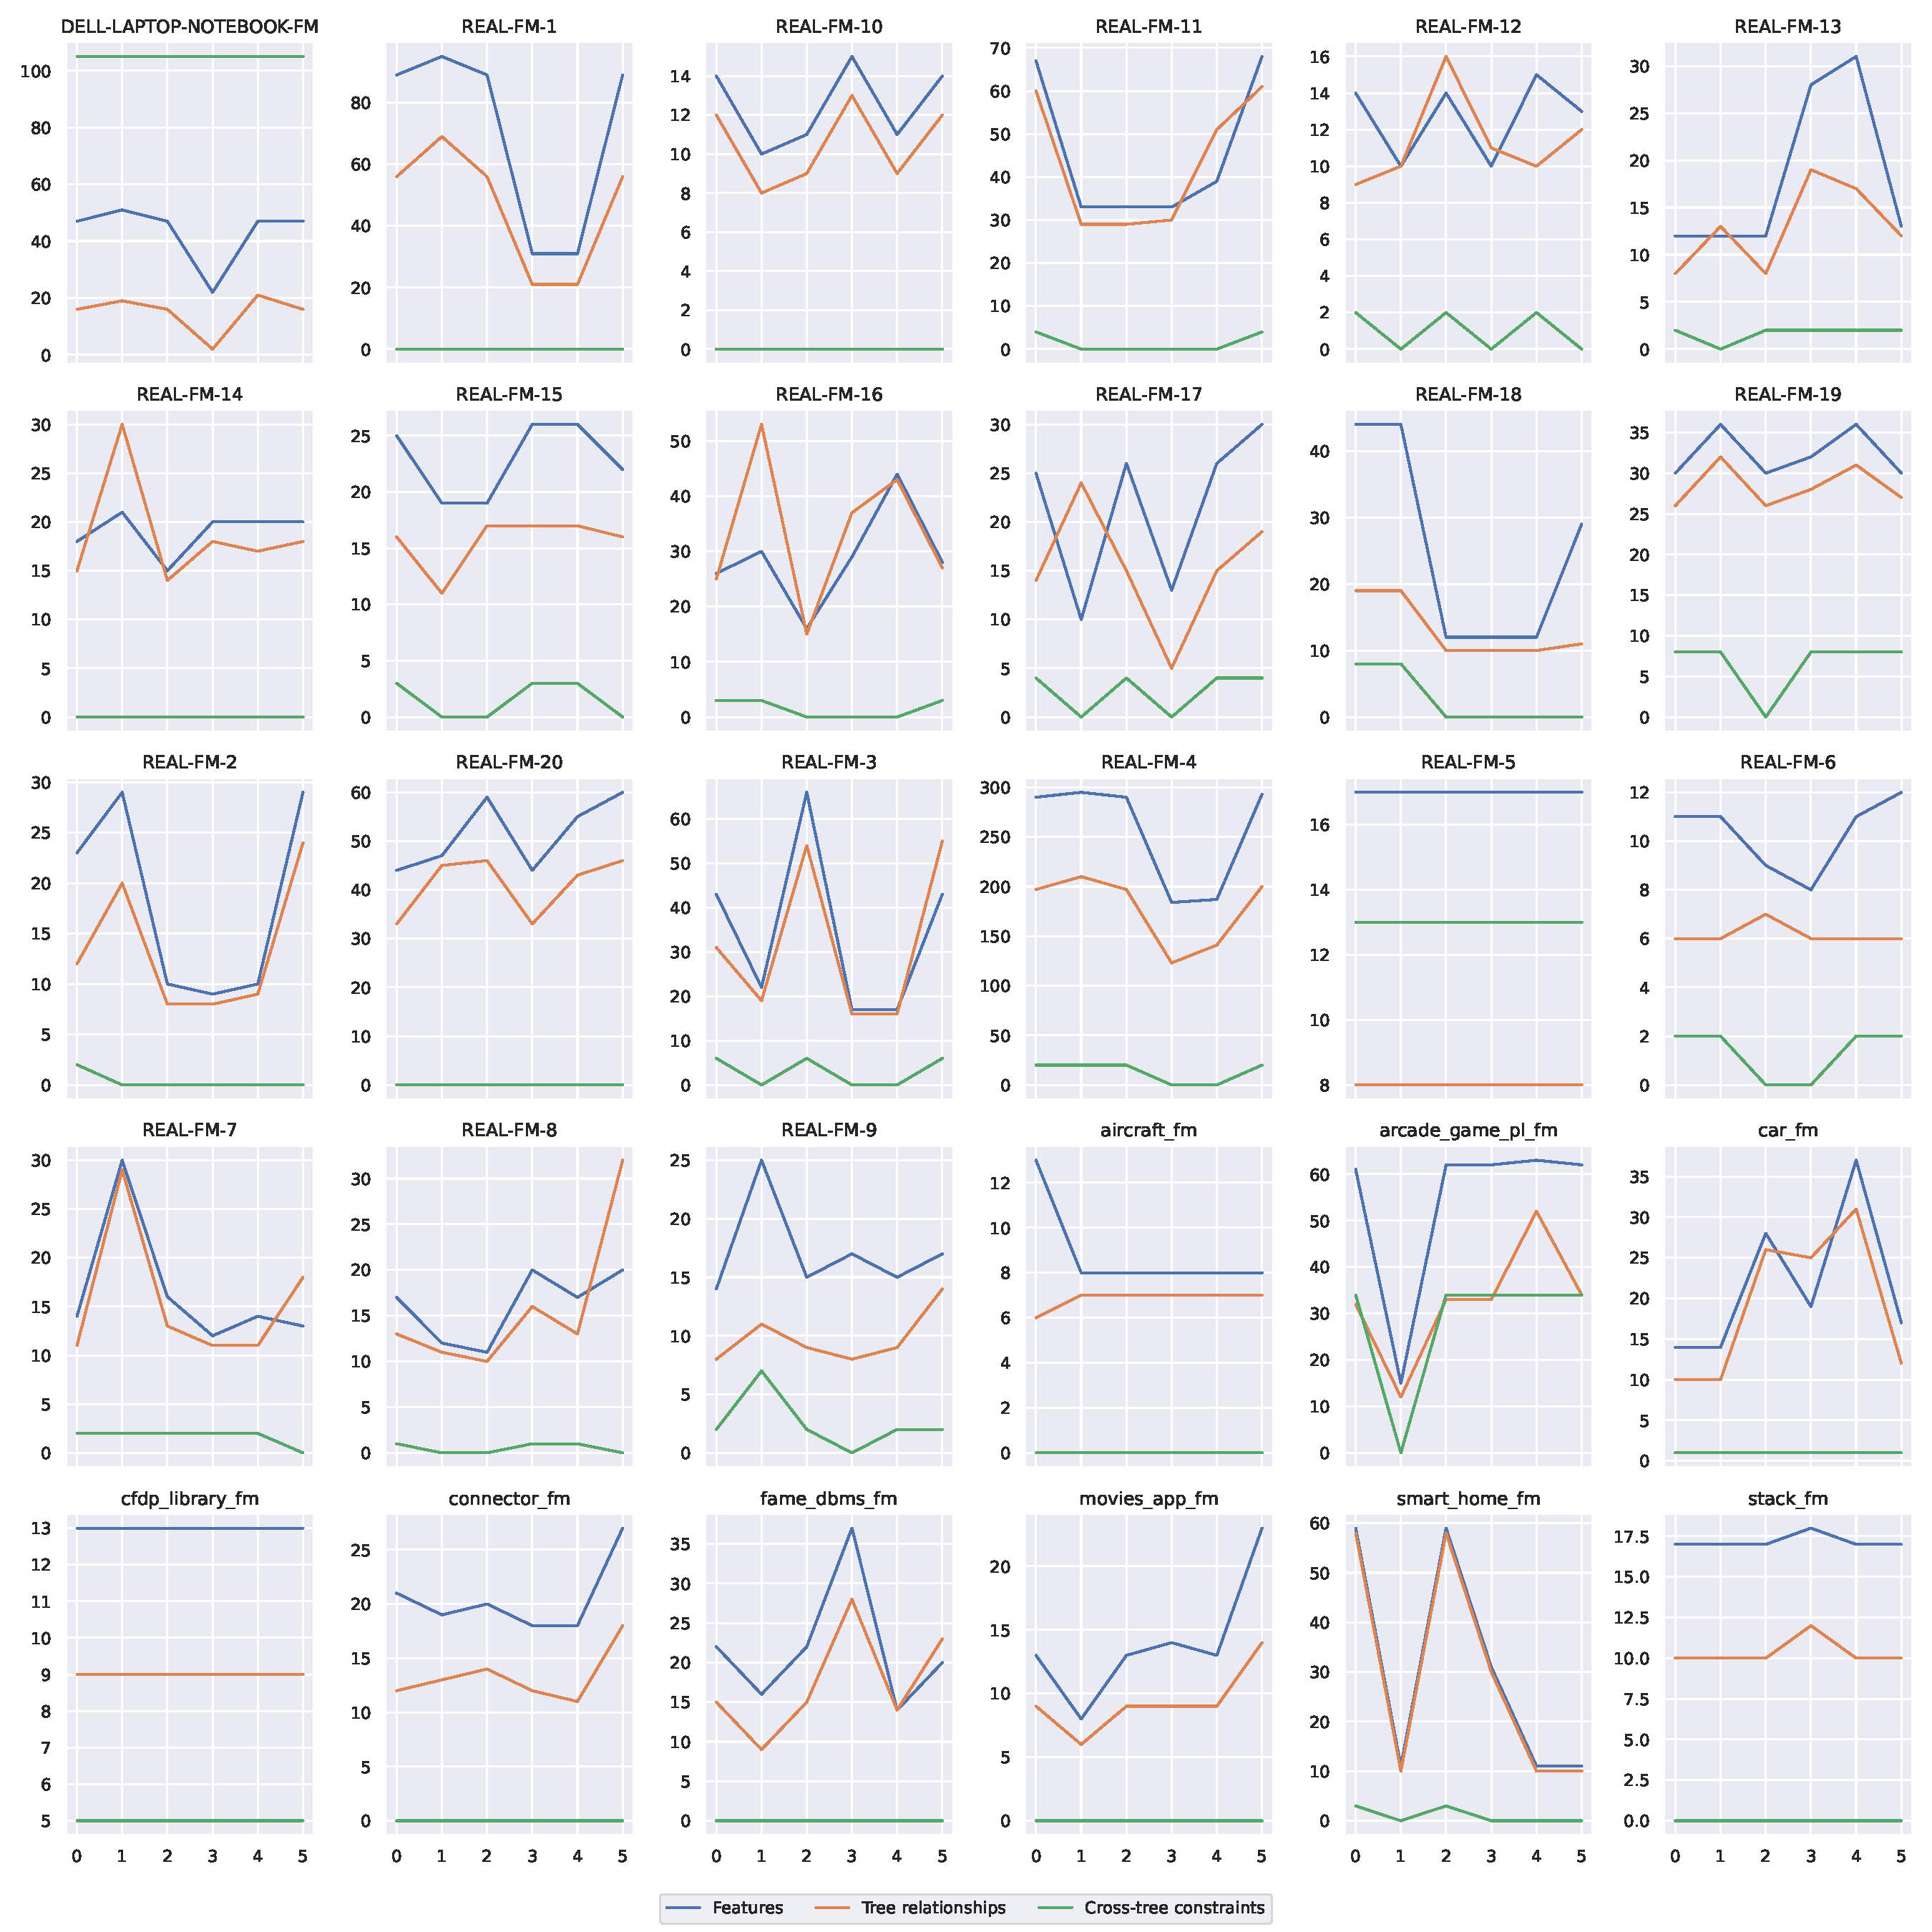
\includegraphics[width=.8\textwidth]{semantics_structure.pdf}
  \caption{Reprodução do experimento 2: features, cross-tree constraints e relações por iteração (0 = original).}
  \label{fig:estrutura}
\end{figure*}

\paragraph{Discrepância na similaridade de domínio.} \todo{discutir: a métrica premia cópias (resposta vazia $\Rightarrow$ 1,0) e penaliza variantes que perdem features; motiva o funil da replicação.}

\section{Desenho da replicação}
\label{sec:replicacao}

\subsection{Questões de pesquisa}
\begin{description}
  \item[\RQ{1}] Os LLMs atuais, via API e local, mantêm a taxa de $\approx$90\% de variantes sintaticamente válidas obtida pelo Codex?
  \item[\RQ{2}] Entre as variantes sintaticamente válidas, quantas são logicamente consistentes (ao menos um produto possível e sem dead features)?
  \item[\RQ{3}] Quantas features e restrições os LLMs acrescentam e removem em relação ao modelo original?
  \item[\RQ{4}] As features acrescentadas mantêm o domínio do modelo original (similaridade de cosseno $\geq 0{,}5$)?
\end{description}

\subsection{Alterações em relação ao estudo original}
\begin{table}[t]
  \caption{Estudo original versus replicação.}
  \label{tab:desenho}
  \small
  \begin{tabular}{p{.17\columnwidth}p{.33\columnwidth}p{.38\columnwidth}}
    \toprule
    & Original & Replicação \\
    \midrule
    LLM & Codex (desativado) & \todo{modelo API} e \todo{modelo local via Ollama} \\
    Pedido & completar a partir da linha 10, sem instrução & instruction prompting com o texto do artigo \\
    Volume & $30\times5=150$ & $2\times30\times5=300$ (+150 do Codex) \\
    Embeddings & Cohere v2 (4096 dims) & Cohere \texttt{embed-english-v3.0} \\
    Avaliação & sintaxe, totais, similaridade & funil: sintaxe, lógica, estrutura, domínio \\
    \bottomrule
  \end{tabular}
\end{table}

\subsection{Prompt}
LLMs atuais de chat não completam o meio de um arquivo; por isso usamos \emph{instruction prompting}, técnica e texto descritos no próprio artigo original: (1)~contexto (``UVL specifies variability models with a tree-like structure\ldots''); (2)~instrução (``Augment the following UVL example while preserving formalism and semantic similarity.''); (3)~o modelo original completo; (4)~formato de saída (acréscimo nosso): devolver apenas o modelo \uvl{} completo. Temperatura 0,7 e top-p 1, como no original. \todo{limite de tokens, seed, datas das execuções, versões dos modelos.}

\subsection{Avaliação em funil}
Cada etapa avalia apenas as variantes aprovadas na anterior: (1)~\textbf{sintaxe} --- parser do \flamapy{}; (2)~\textbf{lógica} --- modelo não vazio e sem dead features (\texttt{fm\_characterization}); (3)~\textbf{estrutura} --- features e restrições acrescentadas/removidas, pela comparação das listas de nomes; (4)~\textbf{domínio} --- similaridade de cosseno $\geq 0{,}5$, calculada apenas para variantes que acrescentaram features sem remover nenhuma, para que cópias (1,0) e perdas não distorçam a medida.

\section{Resultados}
\label{sec:resultados}

\subsection{RQ1: validade sintática}
\todo{tabela: válidas por LLM (Codex, API, local).}

\subsection{RQ2: consistência lógica}
\todo{}

\subsection{RQ3: mudanças estruturais}
\todo{}

\subsection{RQ4: coerência de domínio}
\todo{}

\section{Discussão}
\label{sec:discussao}
\todo{o que confirma/refuta o original; limitações da métrica de similaridade; custo e reprodutibilidade de LLMs fechados vs.\ locais.}

\section{Ameaças à validade}
\label{sec:ameacas}
\paragraph{Validade interna.} \todo{não determinismo dos LLMs (temperatura 0,7); mudança de prompt em relação ao original.}
\paragraph{Validade de construto.} \todo{similaridade de cosseno como proxy de domínio; troca do modelo de embeddings (v2 $\rightarrow$ v3.0).}
\paragraph{Validade externa.} \todo{30 modelos do SPLOT, pequenos; poucos LLMs.}
\paragraph{Confiabilidade.} \todo{versões fixadas; LLMs via API podem mudar ou ser desativados, como o Codex.}

\section{Conclusão}
\label{sec:conclusao}
\todo{}


\section*{Disponibilidade de artefatos}
Código, ambiente fixado, respostas dos LLMs e resultados: \todo{URL do repositório do grupo / Zenodo}. Artefatos originais: \url{https://github.com/diverso-lab/SPLC23-LLM-artefact}.


\bibliographystyle{ACM-Reference-Format}
\bibliography{referencias}

\end{document}
